%
%  Copyright (c) 1995-2015, Regents of the University of Colorado
%
%  All rights reserved.
%
\documentclass[11pt]{article}
\usepackage{makeidx}
\usepackage{graphicx,color}
%\usepackage[pdfpagelabels=false,pageanchor,hyperindex,breaklinks,plainpages=false]{hyperref}
\usepackage[pdfpagelabels=false,pageanchor,hyperindex,plainpages=false]{hyperref}
\newcommand{\eidx}[1]{\index{#1@\emph{#1}}}
\newcommand{\vnumber}{2.7.0}
\title{CUDD: CU Decision Diagram Package\\Release \vnumber}
\author{Fabio Somenzi\\
Department of Electrical, Computer, and Energy Engineering\\
University of Colorado at Boulder\\
$<$Fabio@Colorado.EDU$>$}
\makeindex
\begin{document}
\bibliographystyle{plain}
\maketitle

\tableofcontents
\clearpage

%----------------------------------------
\section{Introduction}
\label{sec:intro}

The CUDD package provides functions to manipulate Binary Decision
Diagrams\index{BDD} (BDDs) \cite{BDD,BBR},
Algebraic Decision Diagrams\index{ADD} (ADDs)
\cite{Bahar93}, and Zero-suppressed Binary Decision
Diagrams\index{ZDD} (ZDDs)
\cite{Minato93}. BDDs are used to represent
switching\index{function!switching} functions; ADDs are used to
represent functions from $\{0,1\}^n$ to an arbitrary set.  ZDDs
represent switching\index{function!switching} functions like BDDs;
however, they are much more efficient than BDDs when the functions to
be represented are characteristic\index{function!characteristic}
functions of cube\index{cube sets} sets, or in general, when the
ON-set\index{function!ON-set} of the function to be represented is
very sparse. They are inferior to BDDs in other cases.

The package provides a large set of operations on BDDs, ADDs, and
ZDDs, functions to convert BDDs into ADDs or ZDDs and vice versa, and
a large assortment of variable reordering\index{reordering} methods.

The CUDD package can be used in three ways:
\begin{itemize}
\item As a black box\index{box!black}.  In this case, the application
  program that needs to manipulate decision diagrams only uses the
  exported functions of the package. The rich set of functions
  included in the CUDD package allows many applications to be written
  in this way.  Section~\ref{sec:user} describes how to use the
  exported functions of the package. An application written in terms
  of the exported functions of the package needs not concern itself
  with the details of variable reordering\index{reordering}, which may
  take place behind the scenes.
\item As a clear box\index{box!clear}. When writing a sophisticated
  application based on decision diagrams, efficiency often dictates
  that some functions be implemented as direct recursive manipulation
  of the diagrams, instead of being written in terms of existing
  primitive functions.  Section~\ref{sec:prog} explains how to add new
  functions to the CUDD package. It also details how to write a
  recursive function that may be interrupted by
  dynamic\index{reordering!dynamic} variable reordering.
\item Through an interface. Object-oriented languages like C++ and
  Perl5 can free the programmer from the burden of memory management.
  A C++ interface is included in the distribution of CUDD. It
  automatically frees decision diagrams that are no longer used by the
  application and overloads operators. Almost all the functionality
  provided by the CUDD exported functions is available through the C++
  interface, which is especially recommended for fast prototyping.
  Section~\ref{sec:cpp} explains how to use the interface. A Perl5
  interface also exists and is ditributed separately. (See
  Section~\ref{sec:getFriends}.)
\end{itemize}
In the following, the reader is supposed to be familiar with the basic
ideas about decision diagrams, as found, for instance, in \cite{BBR}.

%----------------------------------------
\section{How to Get CUDD}
\label{sec:getting}

\subsection{The CUDD Package}
\label{sec:getCUDD}

The CUDD package is available via anonymous FTP\index{FTP} from
vlsi.Colorado.EDU\@.  A compressed tar file named
\texttt{cudd-\vnumber.tar.gz} can be found in directory \texttt{pub}.
Once you have this file,
\begin{quote}
  \tt gzip\index{gzip} -dc cudd-\vnumber.tar.gz | tar xvf -
\end{quote}
will create directory \texttt{cudd-\vnumber} and its subdirectories.
These directories contain the decision diagram package, a few support
libraries\index{libraries}, and a test application based on the
decision diagram package.  There is a README\index{README file} file
with instructions on configuration\index{configuration} and
installation\index{installation} in \texttt{cudd-\vnumber}.  In short,
CUDD uses the GNU Autotools for its build.

Once you have made the libraries and program, you can type
\texttt{make check} to perform a sanity check.  Among other things,
\texttt{make check} executes commands like
\begin{quote}
  \tt cd nanotrav\index{nanotrav} \\
  nanotrav -p 1 -autodyn -reordering sifting -trav mult32a.blif
\end{quote}
This command runs a simple-minded FSM traversal program on a simple
model. (On a reasonable machine, it takes less than 0.5 s.) The output
produced by the program is checked against
\texttt{cudd-\vnumber/nanotrav/mult32a.out}.  More information on the
\texttt{nanotrav\index{nanotrav}} test program can be found in the file
\texttt{cudd-\vnumber/nanotrav/README\index{README file}}.

If you want to be notified of new releases of the CUDD package, send a
message to \texttt{Fabio@Colorado.EDU}.

\subsection{CUDD Friends}
\label{sec:getFriends}

Two CUDD extensions are available via anonymous FTP\index{FTP} from
vlsi.Colorado.EDU\@.
\begin{itemize}
\item \emph{PerlDD} is an object-oriented Perl5 interface to CUDD. It
  is organized as a standard Perl extension module. The Perl interface
  is at a somewhat higher level than the C++ interface, but it is not
  as complete.
\item \emph{DDcal} is a graphic BDD calculator based on CUDD, Perl-Tk,
  and dot. (See Section~\ref{sec:dump} for information on \emph{dot}.)

\end{itemize}
%----------------------------------------
\section{User's Manual}
\label{sec:user}

This section describes the use of the CUDD package as a black box.

\subsection{Compiling and Linking}
\label{sec:compileExt}\index{compiling}

To build an application that uses the CUDD package, you should add
\begin{verbatim}
#include "cudd.h"
\end{verbatim}
\index{cudd.h}
to your source files, and should link
\verb|libcudd.a|\index{libraries!cudd} to your executable.

Keep in mind that whatever flags affect the size of data
structures---for instance the flags used to use 64-bit pointers where
available---must be specified when compiling both CUDD and the files
that include its header files.

\subsection{Basic Data Structures}
\label{sec:struct}

\subsubsection{Nodes}
\label{sec:nodes}

BDDs, ADDs, and ZDDs are made of DdNode's. A DdNode\index{DdNode}
(node\index{node} for short) is a structure with several fields. Those
that are of interest to the application that uses the CUDD package as
a black box are the variable index\index{node!variable index}, the
reference\index{node!reference count} count, and the value. The
remaining fields are pointers that connect nodes among themselves and
that are used to implement the unique\index{table!unique} table. (See
Section~\ref{sec:manager}.)

The \emph{index} field holds the name of the variable that labels the
node. The index of a variable is a permanent attribute that reflects
the order\index{variable!order} of creation.  Index 0 corresponds to
the variable created first. On a machine with 32-bit pointers, the
maximum number of variables is the largest value that can be stored in
an unsigned short integer minus 1. The largest index is reserved for
the constant\index{node!constant} nodes. When 64-bit pointers are
used, the maximum number of variables is the largest value that can be
stored in an unsigned integer minus 1.

When variables are reordered to reduce the size of the decision
diagrams, the variables may shift in the order, but they retain their
indices. The package keeps track of the variable
permutation\index{variable!permutation} (and its inverse). The
application is not affected by variable reordering\index{reordering},
except in the following cases.
\begin{itemize}
\item If the application uses generators\index{generator}
  (\emph{Cudd\_ForeachCube} \eidx{Cudd\_ForeachCube} and
  \emph{Cudd\_ForeachNode}\eidx{Cudd\_ForeachNode}) and reordering is
  enabled, then it must take care not to call any operation that may
  create new nodes (and hence possibly trigger reordering). This is
  because the cubes (i.e., paths) and nodes of a diagram change as a
  result of reordering.
\item If the application uses
  \emph{Cudd\_bddConstrain}\eidx{Cudd\_bddConstrain} and reordering
  takes place, then the property of \emph{Cudd\_bddConstrain} of
  being an image restrictor is lost.
\end{itemize}

The CUDD package relies on garbage\index{garbage collection}
collection to reclaim the memory used by diagrams that are no longer
in use. The scheme employed for garbage collection is based on keeping
a reference\index{node!reference count} count for each node.  The
references that are counted are both the internal references
(references from other nodes) and external references (typically
references from the calling environment).  When an application creates
a new BDD\index{BDD}, ADD\index{ADD}, or ZDD\index{ZDD}, it must
increase its reference count explicitly, through a call to
\emph{Cudd\_Ref}\eidx{Cudd\_Ref}.  Similarly, when a diagram is no
longer needed, the application must call
\emph{Cudd\_RecursiveDeref}\eidx{Cudd\_RecursiveDeref} (for BDDs and
ADDs) or \emph{Cudd\_RecursiveDerefZdd}\eidx{Cudd\_RecursiveDerefZdd}
(for ZDDs) to ``recycle\index{node!recycling}'' the nodes of the
diagram.

Terminal\index{node!constant!value} nodes carry a value. This is especially
important for ADDs.  By default, the value is a double%
\index{floating point!double (C type)}.
To change to something different (e.g., an integer), the
package must be modified and recompiled.  Support for this process is
very rudimentary.

\subsubsection{The Manager}
\index{manager}\label{sec:manager}

All nodes used in BDDs, ADDs, and ZDDs are kept in special
hash\index{table!hash} tables called the
\emph{unique\index{table!unique} tables}.  Specifically, BDDs and ADDs
share the same unique table, whereas ZDDs have their own table.  As
the name implies, the main purpose of the unique table is to guarantee
that each node is unique; that is, there is no other node labeled by
the same variable and with the same children.  This uniqueness
property makes decision diagrams canonical\index{canonical}.  The
unique\index{table!unique} tables and some auxiliary data structures
make up the DdManager\index{DdManager} (manager\index{manager} for
short).  Though the application that uses only the exported functions
needs not be concerned with most details of the manager, it has to
deal with the manager in the following sense. The application must
initialize the manager by calling an appropriate function.  (See
Section~\ref{sec:init}.)  Subsequently, it must pass a pointer to the
manager to all the functions that operate on decision diagrams.

% With the exception of a few statistical counters\index{statistical
%   counters}, there are no global\index{global variables} variables in
% the CUDD package. Therefore, it is possible to have multiple
% managers simultaneously active in the same application.\footnote{The
%   global statistical counters are used locally; hence they are
%   compatible with the use of multiple managers.} It is the pointers to
% the managers that tell the functions on what data they should operate.

\subsubsection{Cache}
\index{cache}\label{sec:memoize}

Efficient recursive manipulation of decision diagrams requires the use
of a table to store computed results. This table\index{table!computed}
is called here the \emph{cache\index{cache}} because it is
effectively handled like a cache of variable but limited capacity. The
CUDD package starts by default with a small cache, and increases its
size until either no further benefit is achieved, or a limit size is
reached. The user can influence this policy by choosing initial and
limit values for the cache size.

Too small a cache will cause frequent overwriting of useful results.
Too large a cache will cause overhead, because the whole cache is
scanned every time garbage\index{garbage collection} collection takes
place. The optimal parameters depend on the specific application. The
default parameters work reasonably well for a large spectrum of
applications.

The cache\index{cache} of the CUDD package is used by most recursive
functions of the package, and can be used by user-supplied functions
as well. (See Section~\ref{sec:cache}.)

\subsection{Initializing and Shutting Down a DdManager}
\index{DdManager}\label{sec:init}

To use the functions in the CUDD package, one has first to initialize
the package itself by calling \emph{Cudd\_Init}\eidx{Cudd\_Init}.
This function takes four parameters:
\begin{itemize}
\item numVars\index{numVars}: It is the initial number of variables
  for BDDs and ADDs. If the total number of variables needed by the
  application is known, then it is slightly more efficient to create a
  manager with that number of variables. If the number is unknown, it
  can be set to 0, or to any other lower bound on the number of
  variables.  Requesting more variables than are actually needed is
  not incorrect, but is not efficient.
\item numVarsZ\index{numVarsZ}: It is the initial number of variables
  for ZDDs. See Sections~\ref{sec:basicZDD} and~\ref{sec:convertZ} for
  a discussion of the value of this argument.
\item numSlots\index{numSlots}: Determines the initial size of each
  subtable\index{subtable} of the unique\index{table!unique} table.
  There is a subtable for each variable.  The size of each subtable is
  dynamically adjusted to reflect the number of nodes.  It is normally
  O.K. to use the default value for this parameter, which is
  CUDD\_UNIQUE\_SLOTS\index{CUDD\_UNIQUE\_SLOTS}.
\item cacheSize\index{cacheSize}: It is the initial size (number of
  entries) of the cache\index{cache}. Its default value is
  CUDD\_CACHE\_SLOTS\index{CUDD\_CACHE\_SLOTS}.
\item maxMemory\index{maxMemory}: It is the target value for the
  maximum memory occupation (in bytes).  The package uses this value to
  decide two parameters.
  \begin{itemize}
  \item the maximum size to which the cache will grow, regardless of
    the hit rate or the size of the unique\index{table!unique} table.
  \item the maximum size to which growth of the unique table will be
    preferred to garbage collection.
  \end{itemize}
  If maxMemory is set to 0, CUDD tries to guess a good value based on
  the available memory.
\end{itemize}
A typical call to \emph{Cudd\_Init}\eidx{Cudd\_Init} may look
like this:
\begin{verbatim}
  manager = Cudd_Init(0,0,CUDD_UNIQUE_SLOTS,CUDD_CACHE_SLOTS,0);
\end{verbatim}
To reclaim all the memory associated with a manager, an application
must call \emph{Cudd\_Quit}\eidx{Cudd\_Quit}.  This is normally
done before exiting.


\subsection{Setting Parameters}
\label{sec:params}

The package provides several functions to set the parameters that
control various functions. For instance, the package has an automatic
way of determining whether a larger unique\index{table!unique} table
would make the application run faster.  In that case, the package
enters a ``fast growth\index{table!growth}'' mode in which resizing of
the unique subtables is favored over garbage\index{garbage collection}
collection. When the unique table reaches a given size, however, the
package returns to the normal ``slow growth'' mode, even though the
conditions that caused the transition to fast growth still prevail.
The limit size for fast growth\index{growth} can be read by
\emph{Cudd\_ReadLooseUpTo}\eidx{Cudd\_ReadLooseUpto} and changed by
\emph{Cudd\_SetLooseUpTo}\eidx{Cudd\_SetLooseUpTo}.  Similar pairs of
functions exist for several other parameters. See also
Section~\ref{sec:stats}.

\subsection{Constant Functions}
\index{node!constant}\label{sec:const}

The CUDD Package defines several constant functions. These functions
are created when the manager\index{manager} is initialized, and are accessible
through the manager itself.

\subsubsection{One, Logic Zero, and Arithmetic Zero}
\index{zero!logical}\index{zero!arithmetic}\label{sec:zero}

The constant\index{node!constant} 1 (returned by
\emph{Cudd\_ReadOne}\eidx{Cudd\_ReadOne}) is common to BDDs, ADDs, and
ZDDs.  However, its meaning is different for ADDs and BDDs, on the one
hand, and ZDDs, on the other hand.  The diagram consisting of the
constant 1 node only represents the constant 1 function for ADDs and
BDDs. For ZDDs, its meaning depends on the number of variables: It is
the conjunction of the complements of all variables.  Conversely, the
representation of the constant 1 function depends on the number of
variables. The constant 1 function of $n$ variables is returned by
\emph{Cudd\_ReadZddOne}\eidx{Cudd\_ReadZddOne}.

The constant 0 is common to ADDs and ZDDs, but not to BDDs.  The
BDD\index{BDD} logic 0 is {\bf not} associated with the constant 0
function: It is obtained by complementation
(\emph{Cudd\_Not}\eidx{Cudd\_Not}) of the constant 1.  (It is also
returned by \emph{Cudd\_ReadLogicZero}\eidx{Cudd\_ReadLogicZero}.)
All other constants are specific to ADDs.

\subsubsection{Predefined Constants}
\label{sec:predef-const}

Besides 0 (returned by \emph{Cudd\_ReadZero}\eidx{Cudd\_ReadZero})
and 1, the following constant\index{node!constant} functions are
created at initialization time.
\begin{enumerate}
\item PlusInfinity\index{PlusInfinity} and
  MinusInfinity\index{MinusInfinity}: On computers implementing the
  IEEE\index{floating point!IEEE Standard 754} standard 754 for
  floating-point\index{floating point} arithmetic, these two constants
  are set to the signed infinities\index{infinities}.  The values of
  these constants are returned by
  \emph{Cudd\_ReadPlusInfinity}\eidx{Cudd\_ReadPlusInfinity} and
  \emph{Cudd\_ReadMinusInfinity}\eidx{Cudd\_ReadMinusInfinity}.
\item Epsilon\index{Epsilon}: This constant, initially set to
  $10^{-12}$, is used in comparing floating point values for equality.
  Its value is returned by the function
  \emph{Cudd\_ReadEpsilon}\eidx{Cudd\_ReadEpsilon}, and it can be
  modified by calling \emph{Cudd\_SetEpsilon}\eidx{Cudd\_SetEpsilon}.
  Unlike the other constants, it does not correspond to a node.
\end{enumerate}

\subsubsection{Background}
\index{background value}\label{sec:background}

The background value is a constant\index{node!constant} typically used
to represent non-existing arcs in graphs. Consider a shortest path
problem. Two nodes that are not connected by an arc can be regarded as
being joined by an arc\index{graph!arc length} of infinite length. In
shortest path problems, it is therefore convenient to set the
background value to PlusInfinity\index{PlusInfinity}. In network flow
problems, on the other hand, two nodes not connected by an arc can be
regarded as joined by an arc\index{graph!arc capacity} of 0 capacity.
For these problems, therefore, it is more convenient to set the
background value to 0.  In general, when representing
sparse\index{matrix!sparse} matrices, the background value is the value that
is assumed implicitly.

At initialization, the background value is set to 0. It can be read
with \emph{Cudd\_ReadBackground}\eidx{Cudd\_ReadBackground}, and
modified with \emph{Cudd\_SetBackground}.  The background value
affects procedures that read sparse matrices and graphs
(like \emph{Cudd\_addRead}\eidx{Cudd\_addRead} and
\emph{Cudd\_addHarwell}\eidx{Cudd\_addHarwell}), procedures that print
out sum-of-product\index{function!sum of products} expressions for
ADDs (\emph{Cudd\_PrintMinterm}\eidx{Cudd\_PrintMinterm}), generators
of cubes (\emph{Cudd\_ForeachCube}\eidx{Cudd\_ForeachCube}), and
procedures that count minterms\index{function!minterms}
(\emph{Cudd\_CountMinterm}\eidx{Cudd\_CountMinterm}).

\subsubsection{New Constants}
\label{sec:newconst}

New constant\index{node!constant} can be created by calling
\emph{Cudd\_addConst}\eidx{Cudd\_addConst}. This function will
retrieve the ADD\index{ADD} for the desired constant, if it already
exist, or it will create a new one.  Obviously, new constants should
only be used when manipulating ADDs.

\subsection{Creating Variables}
\label{sec:newvar}

Decision diagrams are typically created by combining simpler decision
diagrams.  The simplest decision diagrams, of course, cannot be
created in that way.  Constant functions have been discussed in
Section~\ref{sec:const}.  In this section we discuss the simple
variable functions, also known as \emph{projection\index{projection
    functions} functions}.

\subsubsection{New BDD and ADD Variables}
\label{sec:BDDADDvar}

The projection\index{projection functions} functions are distinct for
BDDs and ADDs. A projection function for BDDs consists of an internal
node with both outgoing arcs pointing to the constant 1. The
\emph{else} arc\index{arc!complement} is complemented.

An ADD projection function, on the other hand, has the \emph{else}
pointer directed to the arithmetic\index{zero!arithmetic} zero
function. One should never mix the two types of variables.  BDD
variables should be used when manipulating BDDs, and ADD variables
should be used when manipulating ADDs.  Three functions are provided
to create BDD variables:
\begin{itemize}
\item \emph{Cudd\_bddIthVar}\eidx{Cudd\_bddIthVar}: Returns
  the projection\index{projection functions} function with index $i$.
  If the function does not exist, it is created.
\item \emph{Cudd\_bddNewVar}\eidx{Cudd\_bddNewVar}: Returns a
  new projection\index{projection functions} function, whose index is
  the largest index in use at the time of the call, plus 1.
\item \emph{Cudd\_bddNewVarAtLevel}\eidx{Cudd\_bddNewVarAtLevel}:
  Similar to \emph{Cudd\_bddNewVar}\eidx{Cudd\_bddNewVar}.  In
  addition it allows to specify the position in the variable
  order\index{variable!order} at which the new variable should be
  inserted.  In contrast, \emph{Cudd\_bddNewVar}\eidx{Cudd\_bddNewVar}
  adds the new variable at the end of the order.
\end{itemize}
The analogous functions for ADDs are
\emph{Cudd\_addIthVar}\eidx{Cudd\_addIthVar},
\emph{Cudd\_addNewVar}\eidx{Cudd\_addNewVar}, and
\emph{Cudd\_addNewVarAtLevel}\eidx{Cudd\_addNewVarAtLevel}.

\subsubsection{New ZDD Variables}
\index{ZDD}\label{sec:ZDDvars}

Unlike the projection functions of BDDs and ADDs, the
projection\index{projection functions} functions of ZDDs have diagrams
with $n+1$ nodes, where $n$ is the number of variables.  Therefore the
ZDDs of the projection functions change when new variables are added.
This will be discussed in Section~\ref{sec:basicZDD}.  Here we assume
that the number of variables is fixed. The ZDD of the $i$-th
projection function is returned by
\emph{Cudd\_zddIthVar}\eidx{Cudd\_zddIthVar}.

\subsection{Basic BDD Manipulation}
\index{BDD}\label{sec:basicBDD}

Common manipulations of BDDs can be accomplished by calling
\emph{Cudd\_bddIte}.  This function takes three BDDs, $f$, $g$, and
$h$, as arguments and computes $f\cdot g + f'\cdot h$. Like all the
functions that create new BDDs or ADDs, \emph{Cudd\_bddIte}\eidx{Cudd\_bddIte} returns a result that must be
explicitly referenced by the caller.  \emph{Cudd\_bddIte} can be used
to implement all two-argument Boolean functions.  However, the package
also provides \emph{Cudd\_bddAnd}\eidx{Cudd\_bddAnd} as well as the
other two-operand Boolean functions, which are slightly more efficient
when a two-operand function is called for.  The following fragment of
code illustrates how to build the BDD for the function $f =
x_0'x_1'x_2'x_3'$.
\begin{verbatim}
	DdManager *manager;
	DdNode *f, *var, *tmp;
	int i;

	...

	f = Cudd_ReadOne(manager);
	Cudd_Ref(f);
	for (i = 3; i >= 0; i--) {
	    var = Cudd_bddIthVar(manager,i);
	    tmp = Cudd_bddAnd(manager,Cudd_Not(var),f);
	    Cudd_Ref(tmp);
	    Cudd_RecursiveDeref(manager,f);
	    f = tmp;
	}
\end{verbatim}
This example illustrates the following points:
\begin{itemize}
\item Intermediate results must be ``referenced'' and
  ``dereferenced.''  However, \texttt{var} is a
  projection\index{projection functions} function, and its
  reference\index{node!reference count} count is always greater than
  0.  Therefore, there is no call to \emph{Cudd\_Ref}\eidx{Cudd\_Ref}.
\item The new \texttt{f} must be assigned to a temporary variable
  (\texttt{tmp} in this example).  If the result of
  \emph{Cudd\_bddAnd}\eidx{Cudd\_bddAnd} were assigned directly to
  \texttt{f}, the old \texttt{f} would be lost, and there would be no
  way to free its nodes.
\item The statement \texttt{f = tmp} has the same effect as:
\begin{verbatim}
	    f = tmp;
	    Cudd_Ref(f);
	    Cudd_RecursiveDeref(manager,tmp);
\end{verbatim}
  but is more efficient. The reference\index{node!reference count} is
  ``passed'' from \texttt{tmp} to \texttt{f}, and \texttt{tmp} is now
  ready to be reutilized.
\item It is normally more efficient to build BDDs ``bottom-up.''  This
  is why the loop goes from 3 to 0.  Notice, however, that after
  variable reordering, higher index does not necessarily mean ``closer
  to the bottom.''  Of course, in this simple example, efficiency is
  not a concern.
\item Had we wanted to conjoin the variables in a bottom-up fashion
  even after reordering, we should have used
  \emph{Cudd\_ReadInvPerm}\eidx{Cudd\_ReadInvPerm}.  One has to be
  careful, though, to fix the order of conjunction before entering the
  loop. Otherwise, if reordering takes place, it is possible to use
  one variable twice and skip another variable.
\end{itemize}

\subsection{Basic ADD Manipulation}
\index{ADD}\label{sec:basicADD}

The most common way to manipulate ADDs is via
\emph{Cudd\_addApply}\eidx{Cudd\_addApply}.  This function can apply a
wide variety of operators to a pair of ADDs.  Among the available
operators are addition, multiplication, division, minimum, maximum,
and Boolean operators that work on ADDs whose leaves are restricted to
0 and 1 (0-1 ADDs).

The following fragment of code illustrates how to build the ADD for
the function $f = 5x_0x_1x_2x_3$.
\begin{verbatim}
	DdManager *manager;
	DdNode *f, *var, *tmp;
	int i;

	...

	f = Cudd_addConst(manager,5);
	Cudd_Ref(f);
	for (i = 3; i >= 0; i--) {
	    var = Cudd_addIthVar(manager,i);
	    Cudd_Ref(var);
	    tmp = Cudd_addApply(manager,Cudd_addTimes,var,f);
	    Cudd_Ref(tmp);
	    Cudd_RecursiveDeref(manager,f);
	    Cudd_RecursiveDeref(manager,var);
	    f = tmp;
	}
\end{verbatim}
This example, contrasted to the example of BDD manipulation,
illustrates the following points:
\begin{itemize}
\item The ADD projection\index{projection functions} function are not
  maintained by the manager.  It is therefore necessary to
  reference\index{node!reference} and
  dereference\index{node!dereference} them.
\item The product of two ADDs is computed by calling
  \emph{Cudd\_addApply}\eidx{Cudd\_addApply} with
  \emph{Cudd\_addTimes}\eidx{Cudd\_addTimes} as parameter.  There is
  no ``apply'' function for BDDs, because
  \emph{Cudd\_bddAnd}\eidx{Cudd\_bddAnd} and
  \emph{Cudd\_bddXor}\eidx{Cudd\_bddXor} plus complementation are
  sufficient to implement all two-argument Boolean functions.
\end{itemize}

\subsection{Basic ZDD Manipulation}
\index{ZDD}\label{sec:basicZDD}

ZDDs are often generated by converting\index{conversion!of BDDs to ZDDs}
existing BDDs.  (See Section~\ref{sec:convertZ}.) However, it is also
possible to build ZDDs by applying Boolean operators to other ZDDs,
starting from constants and projection\index{projection functions}
functions.  The following fragment of code illustrates how to build
the ZDD for the function $f = x_0'+x_1'+x_2'+x_3'$. We assume that the
four variables already exist in the manager when the ZDD for $f$ is
built. Note the use of De Morgan's law.
\begin{verbatim}
	DdManager *manager;
	DdNode *f, *var, *tmp;
	int i;

	manager = Cudd_Init(0,4,CUDD_UNIQUE_SLOTS,
			    CUDD_CACHE_SLOTS,0);
	...

	tmp = Cudd_ReadZddOne(manager,0);
	Cudd_Ref(tmp);
	for (i = 3; i >= 0; i--) {
	    var = Cudd_zddIthVar(manager,i);
	    Cudd_Ref(var);
	    f = Cudd_zddIntersect(manager,var,tmp);
	    Cudd_Ref(f);
	    Cudd_RecursiveDerefZdd(manager,tmp);
	    Cudd_RecursiveDerefZdd(manager,var);
	    tmp = f;
	}
	f = Cudd_zddDiff(manager,Cudd_ReadZddOne(manager,0),tmp);
	Cudd_Ref(f);
	Cudd_RecursiveDerefZdd(manager,tmp);
\end{verbatim}
This example illustrates the following points:
\begin{itemize}
\item The projection\index{projection functions} functions are
  referenced, because they are not maintained by the manager.
\item Complementation is obtained by subtracting from the constant 1
  function.
\item The result of \emph{Cudd\_ReadZddOne}\eidx{Cudd\_ReadZddOne}
  does not require referencing.
\end{itemize}
CUDD provides functions for the manipulation of
covers\index{function!cover} represented by ZDDs. For instance,
\emph{Cudd\_zddIsop}\eidx{Cudd\_zddIsop} builds a ZDD representing an
irredundant\index{function!cover!irredundant} sum of products for the
incompletely specified function defined by the two BDDs $L$ and $U$.
\emph{Cudd\_zddWeakDiv}\eidx{Cudd\_zddWeakDiv} performs the weak
division of two covers given as ZDDs.  These functions expect the two
ZDD variables corresponding to the two literals of the function
variable to be adjacent.  One has to create variable groups (see
Section~\ref{sec:reordZ}) for reordering\index{reordering!of ZDDs} of
the ZDD variables to work.  BDD automatic reordering is safe even
without groups: If realignment of ZDD and ADD/BDD variables is
requested (see Section~\ref{sec:consist}) groups will be kept
adjacent.

\subsection{Converting ADDs to BDDs and Vice Versa}
\index{conversion!of ADDs to BDDs}
\index{conversion!of BDDs to ADDs}\label{sec:convert}

Several procedures are provided to convert ADDs to BDDs, according to
different criteria.
(\emph{Cudd\_addBddPattern}\eidx{Cudd\_addBddPattern},
\emph{Cudd\_addBddInterval}\eidx{Cudd\_addBddInterval}, and
\emph{Cudd\_addBddThreshold}\eidx{Cudd\_addBddThreshold}.) The
conversion from BDDs to ADDs
(\emph{Cudd\_BddToAdd}\eidx{Cudd\_BddToAdd}) is based on the simple
principle of mapping the logical 0\index{zero!logical} and 1 on the
arithmetic\index{zero!arithmetic} 0 and 1.  It is also possible to
convert an ADD with integer values (more precisely, floating point
numbers with 0 fractional part) to an array of BDDs by repeatedly
calling \emph{Cudd\_addIthBit}\eidx{Cudd\_addIthBit}.

\subsection{Converting BDDs to ZDDs and Vice Versa}
\index{conversion!of ZDDs to BDDs}
\index{conversion!of BDDs to ZDDs}\label{sec:convertZ}

Many applications first build a set of BDDs and then derive ZDDs from
the BDDs. These applications should create the manager with 0
ZDD\index{ZDD} variables and create the BDDs. Then they should call
\emph{Cudd\_zddVarsFromBddVars}\eidx{Cudd\_zddVarsFromBddVars} to
create the necessary ZDD variables---whose number is likely to be
known once the BDDs are available.  This approach eliminates the
difficulties that arise when the number of ZDD variables changes while
ZDDs are being built.

The simplest conversion from BDDs to ZDDs is a simple change of
representation, which preserves the functions. Simply put, given a BDD
for $f$, a ZDD for $f$ is requested. In this case the correspondence
between the BDD variables and ZDD variables is one-to-one. Hence,
\emph{Cudd\_zddVarsFromBddVars} should be called with the
\emph{multiplicity} parameter equal to 1. The conversion proper can
then be performed by calling
\emph{Cudd\_zddPortFromBdd}\eidx{Cudd\_zddPortFromBdd}. The inverse
transformation is performed by
\emph{Cudd\_zddPortToBdd}\eidx{Cudd\_zddPortToBdd}.

ZDDs are quite often used for the representation of
\emph{covers}\index{function!cover}. This is normally done by
associating two ZDD variables to each variable of the function.  (And
hence, typically, to each BDD variable.)  One ZDD variable is
associated with the positive literal of the BDD variable, while the
other ZDD variable is associated with the negative literal.  A call to
\emph{Cudd\_zddVarsFromBddVars}\eidx{Cudd\_zddVarsFromBddVars} with
\emph{multiplicity} equal to 2 will associate to BDD variable $i$ the
two ZDD variables $2i$ and $2i+1$.

If a BDD variable group tree exists when
\emph{Cudd\_zddVarsFromBddVars} is called (see
Section~\ref{sec:group}) the function generates a ZDD variable group
tree consistent to it.  In any case, all the ZDD variables derived
from the same BDD variable are clustered into a group.

If the ZDD for $f$ is created and later a new ZDD variable is added to
the manager, the function represented by the existing ZDD changes.
Suppose, for instance, that two variables are initially created, and
that the ZDD for $f = x_0 + x_1$ is built. If a third variable is
added, say $x_2$, then the ZDD represents $g = (x_0 + x_1) x_2'$
instead.  This change in function obviously applies regardless of what
use is made of the ZDD\@. However, if the ZDD is used to represent a
cover\index{function!cover}, the cover itself is not changed by the
addition of new variable. (What changes is the
characteristic\index{function!characteristic} function of the cover.)

\subsection{Variable Reordering for BDDs and ADDs}
\index{reordering!of BDDs and ADDs}\label{sec:reorder}

The CUDD package provides a rich set of
dynamic\index{reordering!dynamic} reordering algorithms.  Some of them
are slight variations of existing techniques
\cite{Rudell93,Drechs95,Bollig95,Ishiur91,Plessi93,Jeong93}; some
others have been developed specifically for this package
\cite{Panda94,Panda95b}.

Reordering affects a unique\index{table!unique} table. This means that
BDDs and ADDs, which share the same unique table are simultaneously
reordered. ZDDs, on the other hand, are reordered separately. In the
following we discuss the reordering of BDDs and ADDs. Reordering for
ZDDs is the subject of Section~\ref{sec:reordZ}.

Reordering of the variables can be invoked directly by the application
by calling \emph{Cudd\_ReduceHeap}\eidx{Cudd\_ReduceHeap}. Or it can
be automatically triggered by the package when the number of nodes has
reached a given threshold\index{reordering!threshold}.  (The threshold
is initialized and automatically adjusted after each reordering by the
package.) To enable automatic dynamic reordering (also called
\emph{asynchronous\index{reordering!asynchronous}} dynamic reordering
in this document) the application must call
\emph{Cudd\_AutodynEnable}\eidx{Cudd\_AutodynEnable}.  Automatic
dynamic reordering can subsequently be disabled by calling
\emph{Cudd\_AutodynDisable}\eidx{Cudd\_AutodynDisable}.

All reordering methods are available in both the case of direct call
to \emph{Cudd\_ReduceHeap}\eidx{Cudd\_ReduceHeap} and the case of
automatic invocation.  For many methods, the reordering procedure is
iterated until no further improvement is obtained.  We call these
methods the \emph{converging\index{reordering!converging}} methods.
When constraints are imposed on the relative position of variables
(see Section~\ref{sec:group}) the reordering methods apply inside the
groups.  The groups\index{reordering!group} themselves are reordered
by sifting\index{reordering!sifting}.  Each method is identified by a
constant of the enumerated type
\emph{Cudd\_ReorderingType\index{reordering!Cudd\_ReorderingType}}
defined in \emph{cudd.h\index{cudd.h}} (the external
header\index{header files} file of the CUDD package):

\begin{description}
\item[CUDD\_REORDER\_NONE\index{CUDD\_REORDER\_NONE}:] This method
  causes no reordering.
\item[CUDD\_REORDER\_SAME\index{CUDD\_REORDER\_SAME}:] If passed to
  \emph{Cudd\_AutodynEnable}\eidx{Cudd\_AutodynEnable}, this
  method leaves the current method for automatic reordering unchanged.
  If passed to \emph{Cudd\_ReduceHeap}\eidx{Cudd\_ReduceHeap},
  this method causes the current method for automatic reordering to be
  used.
\item[CUDD\_REORDER\_RANDOM\index{CUDD\_REORDER\_RANDOM}:] Pairs of
  variables are randomly chosen, and swapped in the order. The swap is
  performed by a series of swaps of adjacent variables. The best order
  among those obtained by the series of swaps is retained. The number
  of pairs chosen for swapping\index{reordering!random} equals the
  number of variables in the diagram.
\item[CUDD\_REORDER\_RANDOM\_PIVOT\index{CUDD\_REORDER\_RANDOM\_PIVOT}:]
  Same as CUDD\_REORDER\_RANDOM, but the two variables are chosen so
  that the first is above the variable with the largest number of
  nodes, and the second is below that variable.  In case there are
  several variables tied for the maximum number of nodes, the one
  closest to the root is used.
\item[CUDD\_REORDER\_SIFT\index{CUDD\_REORDER\_SIFT}:] This method is
  an implementation of Rudell's sifting\index{reordering!sifting}
  algorithm \cite{Rudell93}. A simplified description of sifting is as
  follows: Each variable is considered in turn. A variable is moved up
  and down in the order so that it takes all possible positions. The
  best position is identified and the variable is returned to that
  position.

  In reality, things are a bit more complicated. For instance, there
  is a limit on the number of variables that will be sifted. This
  limit can be read with
  \emph{Cudd\_ReadSiftMaxVar}\eidx{Cudd\_ReadSiftMaxVar} and set with
  \emph{Cudd\_SetSiftMaxVar}\eidx{Cudd\_SetSiftMaxVar}.  In addition,
  if the diagram grows too much while moving a variable up or down,
  that movement is terminated before the variable has reached one end
  of the order. The maximum ratio by which the diagram is allowed to
  grow while a variable is being sifted can be read with
  \emph{Cudd\_ReadMaxGrowth}\eidx{Cudd\_ReadMaxGrowth} and set with
  \emph{Cudd\_SetMaxGrowth}\eidx{Cudd\_SetMaxGrowth}.
\item[CUDD\_REORDER\_SIFT\_CONVERGE\index{CUDD\_REORDER\_SIFT\_CONVERGE}:]
  This is the converging\index{reordering!converging} variant of
  CUDD\-\_REORDER\_SIFT.
\item[CUDD\_REORDER\_SYMM\_SIFT\index{CUDD\_REORDER\_SYMM\_SIFT}:]
  This method is an implementation of
  symmetric\index{reordering!symmetric} sifting \cite{Panda94}. It is
  similar to sifting, with one addition: Variables that become
  adjacent during sifting are tested for symmetry\index{symmetry}. If
  they are symmetric, they are linked in a group.  Sifting then
  continues with a group being moved, instead of a single variable.
  After symmetric sifting has been run,
  \emph{Cudd\_SymmProfile}\eidx{Cudd\_SymmProfile} can be called to
  report on the symmetry groups found. (Both positive and negative
  symmetries are reported.)
\item[CUDD\_REORDER\_SYMM\_SIFT\_CONV\index{CUDD\_REORDER\_SYMM\_SIFT\_CONV}:]
  This is the converging\index{reordering!converging} variant of
  CUDD\-\_REORDER\_SYMM\_SIFT.
\item[CUDD\_REORDER\_GROUP\_SIFT\index{CUDD\_REORDER\_GROUP\_SIFT}:]
  This method is an implementation of group\index{reordering!group}
  sifting \cite{Panda95b}. It is similar to symmetric sifting, but
  aggregation\index{aggregation} is not restricted to symmetric
  variables.
\item[CUDD\_REORDER\_GROUP\_SIFT\_CONV\index{CUDD\_REORDER\_GROUP\_SIFT\_CONV}:]
  This method repeats until convergence the combination of
  CUDD\_REORDER\_GROUP\_SIFT and CUDD\-\_REORDER\_WINDOW4.
\item[CUDD\_REORDER\_WINDOW2\index{CUDD\_REORDER\_WINDOW2}:] This
  method implements the window\index{reordering!window} permutation
  approach of Fujita \cite{Fujita91b} and Ishiura \cite{Ishiur91}.
  The size of the window is 2.
\item[CUDD\_REORDER\_WINDOW3\index{CUDD\_REORDER\_WINDOW3}:] Similar
  to CUDD\_REORDER\_WINDOW2, but with a window of size 3.
\item[CUDD\_REORDER\_WINDOW4\index{CUDD\_REORDER\_WINDOW4}:] Similar
  to CUDD\_REORDER\_WINDOW2, but with a window of size 4.
\item[CUDD\_REORDER\_WINDOW2\_CONV\index{CUDD\_REORDER\_WINDOW2\_CONV}:]
  This is the converging\index{reordering!converging} variant of
  CUDD\-\_REORDER\_WINDOW2.
\item[CUDD\_REORDER\_WINDOW3\_CONV\index{CUDD\_REORDER\_WINDOW3\_CONV}:]
  This is the converging variant of CUDD\-\_REORDER\_WINDOW3.
\item[CUDD\_REORDER\_WINDOW4\_CONV\index{CUDD\_REORDER\_WINDOW4\_CONV}:]
  This is the converging variant of CUDD\-\_REORDER\_WINDOW4.
\item[CUDD\_REORDER\_ANNEALING\index{CUDD\_REORDER\_ANNEALING}:] This
  method is an implementation of simulated
  annealing\index{reordering!simulated annealing} for variable
  ordering, vaguely resemblant of the algorithm of \cite{Bollig95}.
  This method is potentially very slow.
\item[CUDD\_REORDER\_GENETIC:\index{CUDD\_REORDER\_GENETIC}] This
  method is an implementation of a genetic\index{reordering!genetic}
  algorithm for variable ordering, inspired by the work of Drechsler
  \cite{Drechs95}. This method is potentially very slow.
\item[CUDD\_REORDER\_EXACT\index{CUDD\_REORDER\_EXACT}:] This method
  implements a dynamic programming approach to
  exact\index{reordering!exact} reordering
  \cite{Held62,Friedman90,Ishiur91}, with improvements described in
  \cite{Jeong93}. It only stores one BDD at the time. Therefore, it is
  relatively efficient in terms of memory.  Compared to other
  reordering strategies, it is very slow, and is not recommended for
  more than 16 variables.
\end{description}
So far we have described methods whereby the package selects an order
automatically. A given order of the variables can also be imposed by
calling \emph{Cudd\_ShuffleHeap}\eidx{Cudd\_ShuffleHeap}.

\subsection{Grouping Variables}
\index{variable!groups}\label{sec:group}

CUDD allows the application to specify constraints on the positions of
group of variables. It is possible to request that a group of
contiguous variables be kept contiguous by the reordering procedures.
It is also possible to request that the relative order of some groups
of variables be left unchanged. The constraints on the order are
specified by means of a tree\index{variable!tree}, which is created in
one of two ways:
\begin{itemize}
\item By calling \emph{Cudd\_MakeTreeNode}\eidx{Cudd\_MakeTreeNode}.
\item By calling the functions of the MTR\index{libraries!mtr} library
  (part of the distribution), and by registering the result with the
  manager using \emph{Cudd\_SetTree}\eidx{Cudd\_SetTree}. The current
  tree registered with the manager can be read with
  \emph{Cudd\_ReadTree}\eidx{Cudd\_ReadTree}.
\end{itemize}

Each node in the tree represents a range of variables. The lower bound
of the range is given by the \emph{low} field of the node, and the
size of the group is given by the \emph{size} field of the
node.\footnote{When the variables in a group are reordered, the
  association between the \emph{low} field and the index of the first
  variable in the group is lost. The package updates the tree to keep
  track of the changes. However, the application cannot rely on
  \emph{low} to determine the position of variables.}  The variables
in each range are kept contiguous. Furthermore, if a node is marked
with the MTR\_FIXED\index{MTR\_FIXED} flag, then the relative order of
the variable ranges associated to its children is not changed.  As an
example, suppose the initial variable order is:
\begin{verbatim}
	x0, y0, z0, x1, y1, z1, ... , x9, y9, z9.
\end{verbatim}
Suppose we want to keep each group of three variables with the same
index (e.g., \verb|x3, y3, z3|) contiguous, while allowing the package
to change the order of the groups. We can accomplish this with the
following code:
\begin{verbatim}
	for (i = 0; i < 10; i++) {
	    (void) Cudd_MakeTreeNode(manager,i*3,3,MTR_DEFAULT);
	}
\end{verbatim}
If we want to keep the order within each group of variables
fixed (i.e., \verb|x| before \verb|y| before \verb|z|) we need to
change MTR\_DEFAULT\index{MTR\_DEFAULT} into MTR\_FIXED.

The \emph{low} parameter passed to
\emph{Cudd\_MakeTreeNode}\eidx{Cudd\_MakeTreeNode} is the index of a
variable (as opposed to its level or position in the order).  The
group tree\index{variable!tree} can be created at any time.  The
result obviously depends on the variable order in effect at creation
time.

It is possible to create a variable group tree also before the
variables themselves are created.  The package assumes in this case
that the index of the variables not yet in existence will equal their
position in the order when they are created.  Therefore, applications
that rely on
\emph{Cudd\_bddNewVarAtLevel}\eidx{Cudd\_bddNewVarAtLevel} or
\emph{Cudd\_addNewVarAtLevel}\eidx{Cudd\_addNewVarAtLevel} to create
new variables have to create the variables before they group them.

The reordering procedure will skip all groups whose variables are not
yet in existence.  For groups that are only partially in existence, the
reordering procedure will try to reorder the variables already
instantiated, without violating the adjacency constraints.


\subsection{Variable Reordering for ZDDs}
\index{reordering!of ZDDs}\label{sec:reordZ}

Reordering of ZDDs is done in much the same way as the reordering of
BDDs and ADDs. The functions corresponding to \emph{Cudd\_ReduceHeap}
and \emph{Cudd\_ShuffleHeap} are
\emph{Cudd\_zddReduceHeap}\eidx{Cudd\_zddReduceHeap} and
\emph{Cudd\_zddShuffleHeap}\eidx{Cudd\_zddShuffleHeap}.  To enable
dynamic\index{reordering!dynamic} reordering, the application must
call \emph{Cudd\_AutodynEnableZdd}\eidx{Cudd\_AutodynEnableZdd}, and
to disable dynamic reordering, it must call
\emph{Cudd\_AutodynDisableZdd}\eidx{Cudd\_AutodynDisableZdd}.  In the
current implementation, however, the choice of reordering methods for
ZDDs is more limited. Specifically, these methods are available:

\begin{description}
\item[CUDD\_REORDER\_NONE\index{CUDD\_REORDER\_NONE};]
\item[CUDD\_REORDER\_SAME\index{CUDD\_REORDER\_SAME};]
\item[CUDD\_REORDER\_RANDOM\index{CUDD\_REORDER\_RANDOM};]
\item[CUDD\_REORDER\_RANDOM\_PIVOT\index{CUDD\_REORDER\_RANDOM\_PIVOT};]
\item[CUDD\_REORDER\_SIFT\index{CUDD\_REORDER\_SIFT};]
\item[CUDD\_REORDER\_SIFT\_CONVERGE\index{CUDD\_REORDER\_SIFT\_CONVERGE};]
\item[CUDD\_REORDER\_SYMM\_SIFT\index{CUDD\_REORDER\_SYMM\_SIFT};]
\item[CUDD\_REORDER\_SYMM\_SIFT\_CONV\index{CUDD\_REORDER\_SYMM\_SIFT\_CONV}.]
\end{description}

To create ZDD variable groups, the application calls
\emph{Cudd\_MakeZddTreeNode}\eidx{Cudd\_MakeZddTreeNode}.

\subsection{Keeping Consistent Variable Orders for BDDs and ZDDs}
\label{sec:consist}

Several applications that manipulate both BDDs and ZDDs benefit from
keeping a fixed correspondence between the order of the BDD variables
and the order of the ZDD variables.  If each BDD variable corresponds
to a group of ZDD variables, then it is often desirable that the
groups of ZDD variables be in the same order as the corresponding BDD
variables.  CUDD allows the ZDD order to track the BDD order and vice
versa. To have the ZDD order track the BDD order, the application
calls \emph{Cudd\_zddRealignEnable}\eidx{Cudd\_zddRealignEnable}.  The
effect of this call can be reversed by calling
\emph{Cudd\_zddRealignDisable}\eidx{Cudd\_zddRealignDisable}.  When
ZDD realignment is in effect, automatic reordering of ZDDs should be
disabled.

\subsection{Hooks}
\index{hook}\label{sec:hooks}

Hooks in CUDD are lists of application-specified functions to be run on
certain occasions. Each hook is identified by a constant of the
enumerated type \emph{Cudd\_HookType}\eidx{Cudd\_HookType}. In Version
\vnumber\ hooks are defined for these occasions:
\begin{itemize}
\item before garbage collection (CUDD\_PRE\_GC\_HOOK);
\item after garbage collection (CUDD\_POST\_GC\_HOOK);
\item before variable reordering (CUDD\_PRE\_REORDERING\_HOOK);
\item after variable reordering (CUDD\_POST\_REORDERING\_HOOK).
\end{itemize}
A function added to a hook receives a pointer to the manager, a
pointer to a constant string, and a pointer to void as arguments; it
must return 1 if successful; 0 otherwise. The second argument is one
of ``DD,'' ``BDD,'' and ``ZDD.'' This allows the hook functions to
tell the type of diagram for which reordering or garbage collection
takes place. The third argument varies depending on the hook. The hook
functions called before or after garbage collection\index{garbage
  collection!hooks} do not use it. The hook functions called before
reordering\index{reordering!hooks} are passed, in addition to the
pointer to the manager, also the method used for reordering. The hook
functions called after reordering are passed the start time. To add a
function to a hook, one uses \emph{Cudd\_AddHook}\eidx{Cudd\_AddHook}.
The function of a given hook are called in the order in which they
were added to the hook.  For sample hook functions, one may look at
\emph{Cudd\_StdPreReordHook}\eidx{Cudd\_StdPreReordHook} and
\emph{Cudd\_StdPostReordHook}\eidx{Cudd\_StdPostReordHook}.

\subsection{Timeouts and Limits}
\index{timeout}\label{sec:timeouts}

It is possible to set a time limit for a manager with
\emph{Cudd\_SetTimeLimit}\eidx{Cudd\_SetTimeLimit}.  Once set, the
time available to the manager can be inspected and modified through
other API functions.
(\emph{Cudd\_TimeLimited}\eidx{Cudd\_TimeLimited},
\emph{Cudd\_ReadTimeLimit}\eidx{Cudd\_ReadTimeLimit},
\emph{Cudd\_UnsetTimeLimit}\eidx{Cudd\_UnsetTimeLimit},
\emph{Cudd\_UpdateTimeLimit}\eidx{Cudd\_UpdateTimeLimit},
\emph{Cudd\_IncreaseTimeLimit}\eidx{Cudd\_IncreaseTimeLimit}.) CUDD
checks for expiration from time to time.  When deadline has
expired, it returns NULL from the call in progress, but it leaves the
manager in a consistent state.  The invoking application must be
designed to handle the NULL values returned.

When reordering, if a timout is approaching, CUDD will quit reordering
to give the application a chance to finish some computation.

It is also possible to invoke some functions that return NULL if they
cannot complete without creating more than a set number of nodes.
See, for instance, \emph{Cudd\_bddAndLimit}\eidx{Cudd\_bddAndLimit}.
Only functions that are documented to check for the number of
generated nodes do so.  (Their names end in ``limit.'')  These
functions set the error code to
\emph{CUDD\_TOO\_MANY\_NODES}\eidx{CUDD\_TOO\_MANY\_NODES} when they
return NULL because of too many nodes.  The error code can be
inspected with \emph{Cudd\_ReadErrorCode}\eidx{Cudd\_ReadErrorCode}
and cleared with
\emph{Cudd\_ClearErrorCode}\eidx{Cudd\_ClearErrorCode}.

\subsection{Writing Decision Diagrams to a File}
\label{sec:dump}

The CUDD package provides several functions to write decision diagrams
to a file. \emph{Cudd\_DumpBlif}\eidx{Cudd\_DumpBlif} writes a
file in \emph{blif} format.  It is restricted to BDDs. The diagrams
are written as a network of multiplexers, one multiplexer for each
internal node of the BDD.

\emph{Cudd\_DumpDot}\eidx{Cudd\_DumpDot} produces input suitable to
the graph-drawing\index{graph!drawing} program
\href{http://www.graphviz.org}{\emph{dot}} written by Eleftherios
Koutsofios and Stephen C. North.  An example of drawing produced by
dot from the output of \emph{Cudd\_DumpDot} is shown in
Figure~\ref{fi:phase}.  \emph{Cudd\_DumpDot} is restricted to BDDs and
ADDs; \emph{Cudd\_zddDumpDot} may be used to draw ZDDs.
\begin{figure}
  \centerline{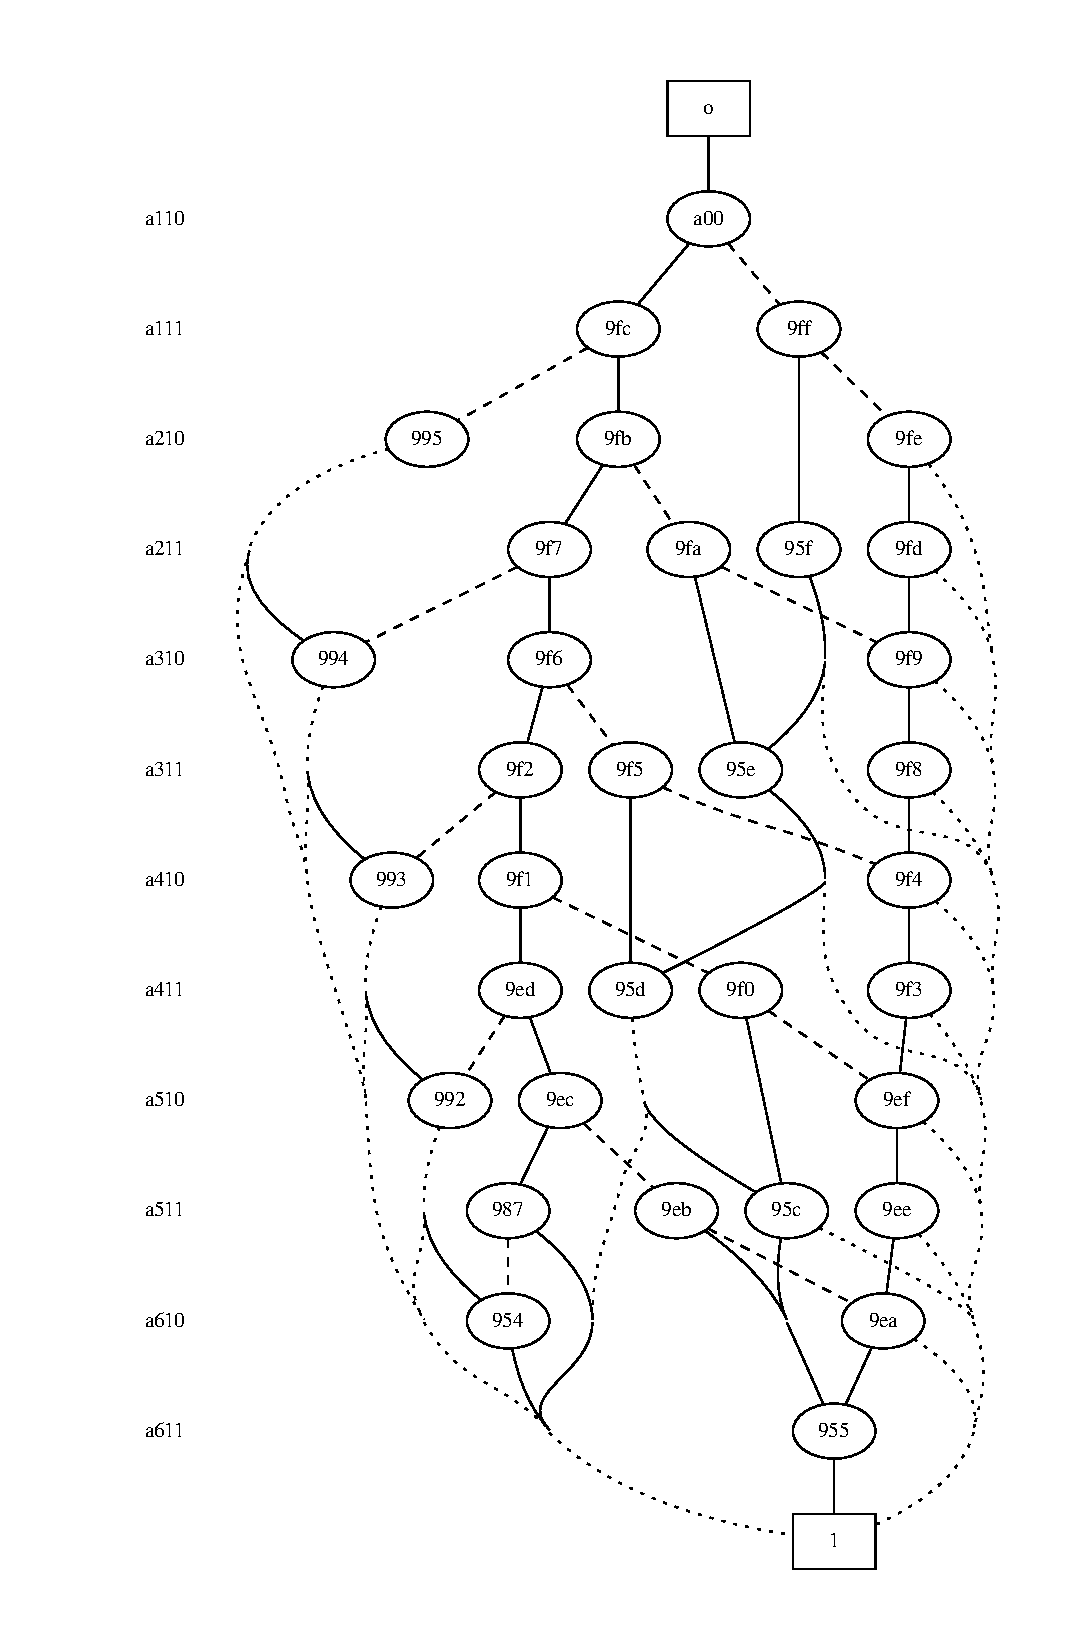
\includegraphics[height=15.5cm]{../doc/phase.pdf}}
\caption{A BDD representing a phase constraint for the optimization of
  fixed-polarity Reed-Muller forms. The label of each node is the
  unique part of the node address. All nodes on the same level
  correspond to the same variable, whose name is shown at the left of
  the diagram. Dotted lines indicate complement\index{arc!complement}
  arcs. Dashed lines indicate regular\index{arc!regular} ``else''
  arcs.\label{fi:phase}}
\end{figure}
\emph{Cudd\_zddDumpDot}\eidx{Cudd\_zddDumpDot} is the analog of
\emph{Cudd\_DumpDot} for ZDDs.

\emph{Cudd\_DumpDaVinci}\eidx{Cudd\_DumpDaVinci} produces input
suitable to the graph-drawing\index{graph!drawing} program
\href{ftp://ftp.uni-bremen.de/pub/graphics/daVinci}{\emph{daVinci}}
developed at the University of Bremen. It is restricted to BDDs and
ADDs.

Functions are also available to produce the input format of
\emph{DDcal} (see Section~\ref{sec:getFriends}) and factored forms.


\subsection{Saving and Restoring BDDs}
\label{sec:save-restore}

The \href{ftp://ftp.polito.it/pub/research/dddmp/}{\emph{dddmp}}
library\index{libraries!dddmp} by Gianpiero Cabodi and Stefano Quer
allows a CUDD application to save BDDs to disk in compact form for
later retrieval.  See the library's own documentation for the details.

%----------------------------------------
\section{Programmer's Manual}
\label{sec:prog}

This section provides additional detail on the workings of the CUDD
package and on the programming conventions followed in its writing.
The additional detail should help those who want to write procedures
that directly manipulate the CUDD data structures.

\subsection{Compiling and Linking}
\index{compiling}\label{sec:compileInt}

If you plan to use the CUDD package as a clear box\index{box!clear}
(for instance, you want to write a procedure that traverses a decision
diagram) you need to add
\begin{verbatim}
#include "cuddInt.h"
\end{verbatim}
to your source files. In addition, you should link \verb|libcudd.a| to
your executable.  Some platforms require specific compiler and linker
flags.  Refer to the \texttt{Makefile} in the top level directory of
the distribution.

\subsection{Reference Counts}
\index{node!reference count}\label{sec:ref}

Garbage\index{garbage collection} collection in the CUDD package is
based on reference counts.  Each node stores the sum of the external
references and internal references. An internal BDD or ADD node is
created by a call to \emph{cuddUniqueInter}\eidx{cuddUniqueInter}, an
internal ZDD node is created by a call to
\emph{cuddUniqueInterZdd}\eidx{cuddUniqueInterZdd}, and a
terminal\index{node!constant} node is created by a call to
\emph{cuddUniqueConst}\eidx{cuddUniqueConst}. If the node returned by
these functions is new, its reference count is zero.  The function
that calls \emph{cuddUniqueInter}\eidx{cuddUniqueInter},
\emph{cuddUniqueInterZdd}\eidx{cuddUniqueInterZdd}, or
\emph{cuddUniqueConst}\eidx{cuddUniqueConst} is responsible for
increasing the reference count of the node.  This is accomplished by
calling \emph{Cudd\_Ref}\eidx{Cudd\_Ref}.

When a function is no longer needed by an application, the memory used
by its diagram can be recycled by calling
\emph{Cudd\_RecursiveDeref}\eidx{Cudd\_RecursiveDeref} (BDDs and ADDs)
or \emph{Cudd\_RecursiveDerefZdd}\eidx{Cudd\_RecursiveDerefZdd}
(ZDDs).  These functions decrease the reference \index{node!reference
  count} count of the node passed to them.  If the reference count
becomes 0, then two things happen:
\begin{enumerate}
\item The node is declared ``dead\index{node!dead};'' this entails
  increasing the counters\index{statistical counters} of the dead
  nodes. (One counter for the subtable\index{subtable} to which the
  node belongs, and one global counter for the
  unique\index{table!unique} table to which the node belongs.) The
  node itself is not affected.
\item The function is recursively called on the two children of the
  node.
\end{enumerate}
For instance, if the diagram of a function does not share any nodes
with other diagrams, then calling
\emph{Cudd\_RecursiveDeref}\eidx{Cudd\_RecursiveDeref} or
\emph{Cudd\_RecursiveDerefZdd}\eidx{Cudd\_RecursiveDerefZdd} on its
root will cause all the nodes of the diagram to become dead.

When the number of dead nodes reaches a given level (dynamically
determined by the package) garbage collection takes place. During
garbage\index{garbage collection} collection dead nodes are returned
to the node free list\index{free list}.

When a new node is created, it is important to increase its
reference\index{node!reference count} count before one of the two
following events occurs:
\begin{enumerate}
\item A call to \emph{cuddUniqueInter}\eidx{cuddUniqueInter},
  to \emph{cuddUniqueInterZdd}\eidx{cuddUniqueInterZdd}, to
  \emph{cuddUniqueConst}\eidx{cuddUniqueConst}, or to a
  function that may eventually cause a call to them.
\item A call to
  \emph{Cudd\_RecursiveDeref}\eidx{Cudd\_RecursiveDeref}, to
  \emph{Cudd\_RecursiveDerefZdd}\eidx{Cudd\_RecursiveDerefZdd}, or to
  a function that may eventually cause a call to them.
\end{enumerate}
In practice, it is recommended to increase the reference count as soon
as the returned pointer has been tested for not being NULL.

\subsubsection{NULL Return Values}
\label{sec:null}

The interface to the memory management functions (e.g., malloc) used
by CUDD intercepts NULL return values and calls a handler.  The
default handler exits with an error message.  If the application does
not install another handler, therefore, a NULL return value from an
exported function of CUDD signals an internal error.

If the aplication, however, installs another handler that lets
execution continue, a NULL pointer returned by an exported function
typically indicates that the process has run out of memory.
\emph{Cudd\_ReadErrorCode}\eidx{Cudd\_ReadErrorCode} can be used to
ascertain the nature of the problem.

An application that tests for the result being NULL can try some
remedial action, if it runs out of memory.  For instance, it may free
some memory that is not strictly necessary, or try a slower algorithm
that takes less space. As an example, CUDD overrides the default
handler when trying to enlarge the cache or increase the number of
slots of the unique table. If the allocation fails, the package prints
out a message and continues without resizing the cache.

\subsubsection{\emph{Cudd\_RecursiveDeref} vs.\ \emph{Cudd\_Deref}}
\label{sec:deref}

It is often the case that a recursive procedure has to protect the
result it is going to return, while it disposes of intermediate
results.  (See the previous discussion on when to increase reference
counts.)  Once the intermediate results have been properly disposed
of, the final result must be returned to its pristine state, in which
the root node may have a reference count of 0. One cannot use
\emph{Cudd\_RecursiveDeref}\eidx{Cudd\_RecursiveDeref} (or
\emph{Cudd\_RecursiveDerefZdd}) for this purpose, because it may
erroneously make some nodes dead.  Therefore, the package provides a
different function: \emph{Cudd\_Deref}\eidx{Cudd\_Deref}. This
function is not recursive, and does not change the dead node counts.
Its use is almost exclusively the one just described: Decreasing the
reference count of the root of the final result before returning from
a recursive procedure.

\subsubsection{When Increasing the Reference Count is Unnecessary}
\index{node!reference count}\label{sec:noref}

When a copy of a predefined constant\index{node!constant} or of a
simple BDD variable is needed for comparison purposes, then calling
\emph{Cudd\_Ref}\eidx{Cudd\_Ref} is not necessary, because these
simple functions are guaranteed to have reference counts greater than
0 at all times. If no call to \emph{Cudd\_Ref} is made, then no
attempt to free the diagram by calling
\emph{Cudd\_RecursiveDeref}\eidx{Cudd\_RecursiveDeref} or
\emph{Cudd\_RecursiveDerefZdd}\eidx{Cudd\_RecursiveDerefZdd} should be
made.

\subsubsection{Saturating Increments and Decrements}
\index{saturating!increments}\index{saturating!decrements}\label{sec:satur}

On 32-bit machines, the CUDD package stores the
reference\index{node!reference count} counts in unsigned short int's.
For large diagrams, it is possible for some reference counts to exceed
the capacity of an unsigned short int.  Therefore, increments and
decrements of reference counts are \emph{saturating}. This means that
once a reference count has reached the maximum possible value, it is
no longer changed by calls to \emph{Cudd\_Ref},
\emph{Cudd\_RecursiveDeref}\eidx{Cudd\_RecursiveDeref},
\emph{Cudd\_RecursiveDerefZdd}\eidx{Cudd\_RecursiveDerefZdd}, or
\emph{Cudd\_Deref}\eidx{Cudd\_Deref}.  As a consequence, some nodes
that have no references may not be declared dead. This may result in a
small waste of memory, which is normally more than offset by the
reduction in size of the node structure.

When using 64-bit pointers, there is normally no memory advantage from
using short int's instead of int's in a DdNode.  Therefore, increments
and decrements are not saturating in that case.  What option is in
effect depends on two macros, SIZEOF\_VOID\_P\index{SIZEOF\_VOID\_P}
and SIZEOF\_INT\index{SIZEOF\_INT}, defined in the configuration
header\index{header files} file (\emph{config.h}\index{config.h}).
The increments and decrements of the reference counts are performed
using two macros: \emph{cuddSatInc}\eidx{cuddSatInc} and
\emph{cuddSatDec}\eidx{cuddSatDec}, whose definitions depend on
SIZEOF\_VOID\_P\index{SIZEOF\_VOID\_P} and
SIZEOF\_INT\index{SIZEOF\_INT}.

\subsection{Complement Arcs}
\index{arc!complement}\label{sec:compl}

If ADDs are restricted to use only the constants 0 and 1, they behave
like BDDs without complement arcs. It is normally easier to write code
that manipulates 0-1 ADDs, than to write code for BDDs. However,
complementation is trivial with complement arcs, and is not trivial
without. As a consequence, with complement arcs it is possible to
check for more terminal cases and it is possible to apply De Morgan's
laws to reduce problems that are essentially identical to a standard
form. This in turn increases the utilization of the cache\index{cache}.

The complement attribute is stored in the least significant bit of the
``else'' pointer of each node. An external pointer to a function can
also be complemented. The ``then'' pointer to a node, on the other
hand, is always \emph{regular\index{arc!regular}}.  It is a mistake to
use a complement\index{arc!complement} pointer as it is to address
memory.  Instead, it is always necessary to obtain a regular version
of it.  This is normally done by calling
\emph{Cudd\_Regular}\eidx{Cudd\_Regular}.  It is also a mistake to
call \emph{cuddUniqueInter}\eidx{cuddUniqueInter} with a complemented
``then'' child as argument.  The calling procedure must apply De
Morgan's laws by complementing both pointers passed to
\emph{cuddUniqueInter}\eidx{cuddUniqueInter} and then taking the
complement of the result.

\subsection{The Cache}
\index{cache}\label{sec:cache}

Each entry of the cache consists of five fields: The operator, three
pointers to operands and a pointer to the result. The operator and the
three pointers to the operands are combined to form three words. The
combination relies on two facts:
\begin{itemize}
\item Most operations have one or two operands. A few bits are
  sufficient to discriminate all three-operands operations.
\item All nodes are aligned to 16-byte boundaries. (32-byte boundaries
  if 64-bit pointers are used.) Hence, there are a few bits available
  to distinguish the three-operand operations from te others and to
  assign unique codes to them.
\end{itemize}

The cache does not contribute to the reference
\index{node!reference count}
counts of the nodes.  The fact that the cache contains a
pointer to a node does not imply that the node is alive. Instead, when
garbage\index{garbage collection} collection takes place, all entries
of the cache pointing to dead\index{node!dead} nodes are cleared.

The cache is also cleared (of all entries) when dynamic
reordering\index{reordering} takes place. In both cases, the entries
removed from the cache are about to become invalid.

All operands and results in a cache entry must be pointers to
DdNodes\index{DdNode}.  If a function produces more than one result,
or uses more than three arguments, there are currently two solutions:
\begin{itemize}
\item Build a separate, local, cache\index{cache!local}. (Using, for
  instance, the \emph{st} library\index{libraries!st}.)
\item Combine multiple results, or multiple operands, into a single
  diagram, by building a ``multiplexing structure'' with reserved
  variables.
\end{itemize}
Support of the former solution is under development. (See
\texttt{cuddLCache.c}..)  Support for the latter solution may be
provided in future versions of the package.

There are three sets of interface\index{interface!cache} functions to
the cache. The first set is for functions with three operands:
\emph{cuddCacheInsert}\eidx{cuddCacheInsert} and
\emph{cuddCacheLookup}\eidx{cuddCacheLookup}. The second set is for
functions with two operands:
\emph{cuddCacheInsert2}\eidx{cuddCacheInsert2} and
\emph{cuddCacheLookup2}\eidx{cuddCacheLookup2}.  The second set is for
functions with one operand:
\emph{cuddCacheInsert1}\eidx{cuddCacheInsert1} and
\emph{cuddCacheLookup1}\eidx{cuddCacheLookup1}.  The second set is
slightly faster than the first, and the third set is slightly faster
than the second.

\subsubsection{Cache Sizing}
\index{cache!sizing}\label{sec:cache-sizing}

The size of the cache can increase during the execution of an
application. (There is currently no way to decrease the size of the
cache, though it would not be difficult to do it.) When a cache miss
occurs, the package uses the following criteria to decide whether to
resize the cache:
\begin{enumerate}
\item If the cache already exceeds the limit given by the
  \texttt{maxCache\index{maxCache}} field of the manager, no resizing
  takes place.  The limit is the minimum of two values: a value set at
  initialization time and possibly modified by the application, which
  constitutes the hard limit beyond which the cache will never grow;
  and a number that depends on the current total number of slots in
  the unique\index{table!unique} table.
\item If the cache is not too large already, resizing is decided based
  on the hit rate. The policy adopted by the CUDD package is
  ``reward-based\index{cache!reward-based resizing}.'' If the cache hit
  rate is high, then it is worthwhile to increase the size of the
  cache.
\end{enumerate}
When resizing takes place, the statistical counters \index{statistical
  counters} used to compute the hit rate are reinitialized so as to
prevent immediate resizing. The number of entries is doubled.

The rationale for the ``reward-based\index{cache!reward-based resizing}''
policy is as follows. In many BDD/ADD applications the hit rate is
not very sensitive to the size of the cache: It is primarily a
function of the problem instance at hand.  If a large hit rate is
observed, chances are that by using a large cache, the results of
large problems (those that would take longer to solve) will survive in
the cache without being overwritten long enough to cause a valuable
cache hit. Notice that when a large problem is solved more than once,
so are its recursively generated subproblems.  If the hit rate is
low, the probability of large problems being solved more than once is
low.

The other observation about the cache sizing policy is that there is
little point in keeping a cache which is much larger than the unique
table. Every time the unique table ``fills up,'' garbage collection is
invoked and the cache is cleared of all dead entries. A cache that is
much larger than the unique\index{table!unique} table is therefore
less than fully utilized.

\subsubsection{Local Caches}
\index{cache!local}\label{sec:local-caches}

Sometimes it may be necessary or convenient to use a local cache.  A
local cache can be lossless\index{cache!lossless} (no results are ever
overwritten), or it may store objects for which
canonical\index{canonical} representations are not available.  One
important fact to keep in mind when using a local cache is that local
caches are not cleared during garbage\index{garbage collection}
collection or before reordering. Therefore, it is necessary to
increment the reference\index{node!reference count} count of all nodes
pointed by a local cache. (Unless their reference counts are
guaranteed positive in some other way. One such way is by including
all partial results in the global result.) Before disposing of the
local cache, all elements stored in it must be passed to
\emph{Cudd\_RecursiveDeref}\eidx{Cudd\_RecursiveDeref}. As consequence
of the fact that all results in a local cache are referenced, it is
generally convenient to store in the local cache also the result of
trivial problems, which are not usually stored in the global cache.
Otherwise, after a recursive call, it is difficult to tell whether the
result is in the cache, and therefore referenced, or not in the cache,
and therefore not referenced.

An alternative approach to referencing the results in the local caches
is to install hook functions (see Section~\ref{sec:hooks}) to be
executed before garbage collection.

\subsection{The Unique Table}
\index{table!unique}\label{sec:unique}

A recursive procedure typically splits the operands by expanding with
respect to the topmost variable. Topmost in this context refers to the
variable that is closest to the roots in the current variable order.
The nodes, on the other hand, hold the index, which is invariant with
reordering. Therefore, when splitting, one must use the
permutation\index{variable!permutation} array maintained by the
package to get the right level. Access to the permutation array is
provided by the macro \emph{cuddI}\eidx{cuddI} for BDDs and ADDs,
and by the macro \emph{cuddIZ}\eidx{cuddIZ} for ZDDs.

The unique table consists of as many hash\index{table!hash} tables as
there are variables in use. These has tables are called \emph{unique
  subtables}.  The sizes of the unique subtables are determined by two
criteria:
\begin{enumerate}
\item The collision\index{cache!collision list} lists should be short
  to keep access time down.
\item There should be enough room for dead\index{node!dead} nodes, to
  prevent too frequent garbage\index{garbage collection} collections.
\end{enumerate}
While the first criterion is fairly straightforward to implement, the
second leaves more room to creativity. The CUDD package tries to
figure out whether more dead node should be allowed to increase
performance.  (See also Section~\ref{sec:params}.) There are two
reasons for not doing garbage collection too often. The obvious one is
that it is expensive.  The second is that dead nodes may be
reclaimed\index{node!reclaimed}, if they are the result of a
successful cache lookup. Hence dead nodes may provide a substantial
speed-up if they are kept around long enough.  The usefulness of
keeping many dead nodes around varies from application to application,
and from problem instance to problem instance. As in the sizing of the
cache, the CUDD package adopts a
``reward-based\index{table!unique!reward-based resizing}'' policy to
decide how much room should be used for the unique table. If the
number of dead nodes reclaimed is large compared to the number of
nodes directly requested from the memory manager, then the CUDD
package assumes that it will be beneficial to allow more room for the
subtables, thereby reducing the frequency of garbage collection.  The
package does so by switching between two modes of operation:
\begin{enumerate}
\item Fast growth\index{table!unique!fast growth}: In this mode, the
  ratio of dead nodes to total nodes required for garbage collection
  is higher than in the slow growth mode to favor resizing
  of the subtables.
\item Slow growth\index{table!unique!slow growth}: In this
  mode keeping many dead nodes around is not as important as
  keeping memory requirements low.
\end{enumerate}
Switching from one mode to the other is based on the following
criteria:
\begin{enumerate}
\item If the unique table is already large, only slow growth is
  possible.
\item If the table is small and many dead nodes are being reclaimed,
  then fast growth is selected.
\end{enumerate}
This policy is especially effective when the diagrams being
manipulated have lots of recombination. Notice the interplay of the
cache sizing and unique sizing: Fast growth normally occurs when the
cache hit rate is large. The cache and the unique table then grow in
concert, preserving a healthy balance between their sizes.

\subsection{Allowing Asynchronous Reordering}
\index{reordering!asynchronous}\label{sec:async}

Asynchronous reordering is the reordering that is triggered
automatically by the increase of the number of nodes. Asynchronous
reordering takes place when a new internal node must be created, and
the number of nodes has reached a given
threshold\index{reordering!threshold}. (The threshold is adjusted by
the package every time reordering takes place.)

Those procedures that do not create new nodes (e.g., procedures that
count the number of nodes or minterms\index{function!minterms}) need
not worry about asynchronous reordering: No special precaution is
necessary in writing them.

Procedures that only manipulate decision diagrams through the exported
functions of the CUDD package also need not concern themselves with
asynchronous reordering. (See Section~\ref{sec:nodes} for the
exceptions.)

The remaining class of procedures is composed of functions that visit
the diagrams and may create new nodes. All such procedures in the CUDD
package are written so that they can be interrupted by dynamic
reordering. The general approach followed goes under the name of
``abort and retry\index{reordering!abort and retry}.'' As the name
implies, a computation that is interrupted by dynamic reordering is
aborted and tried again.

A recursive procedure that can be interrupted by dynamic reordering
(an interruptible\index{reordering!interruptible procedure} procedure
from now on) is composed of two functions.  One is responsible for the
real computation. The other is a simple
wrapper\index{reordering!function wrapper}, which tests whether
reordering occurred and restarts the computation if it did.

Asynchronous reordering of BDDs and ADDs can only be triggered inside
\emph{cuddUniqueInter}\eidx{cuddUniqueInter}, when a new node is about
to be created.  Likewise, asynchronous reordering of ZDDs can only be
triggered inside \emph{cuddUniqueInterZdd}\eidx{cuddUniqueInterZdd}.
When reordering is triggered, three things happen:
\begin{enumerate}
\item \emph{cuddUniqueInter}\eidx{cuddUniqueInter} returns a NULL
  value;
\item The flag \emph{reordered} of the manager is set to 1. (0 means
  no reordering, while 2 indicates an error occurred during
  reordering.)
\item The counter \emph{reorderings} of the manager is incremented.
  The counter is initialized to 0 when the manager is started and can
  be accessed by calling
  \emph{Cudd\_ReadReorderings}\eidx{Cudd\_ReadReorderings}. By taking
  two readings of the counter, an application can determine if
  variable reordering has taken place between the first and the second
  reading.  The package itself, however, does not make use of the
  counter: It is mentioned here for completeness.
\end{enumerate}

The recursive procedure that receives a NULL value from
\emph{cuddUniqueInter}\eidx{cuddUniqueInter} must free all
intermediate results that it may have computed before, and return NULL
in its turn.

The wrapper\index{reordering!function wrapper} function does not
decide whether reordering occurred based on the NULL return value,
because the NULL value may be the result of lack of memory. Instead,
it checks the \emph{reordered} flag.

When a recursive procedure calls another recursive procedure that may
cause reordering, it should bypass the wrapper and call the recursive
procedure directly. Otherwise, the calling procedure will not know
whether reordering occurred, and will not be able to restart.  This is
the main reason why most recursive procedures are internal, rather
than static. (The wrappers, on the other hand, are mostly exported.)

\subsection{Debugging}
\index{debugging}\label{sec:debug}

By defining the symbol DD\_DEBUG\index{DD\_DEBUG} during compilation,
numerous checks are added to the code.  In addition, the procedures
\emph{Cudd\_DebugCheck}\eidx{Cudd\_DebugCheck},
\emph{Cudd\_CheckKeys}\eidx{Cudd\_CheckKeys}, and
\emph{cuddHeapProfile}\eidx{cuddHeapProfile} can be called at any
point to verify the consistency of the data structure.
(\emph{cuddHeapProfile} is an internal procedure.  It is declared in
\emph{cuddInt.h}\index{cuddInt.h}.)  Procedures
\emph{Cudd\_DebugCheck} and \emph{Cudd\_CheckKeys} are especially
useful when CUDD reports that during garbage collection the number of
nodes actually deleted from the unique table is different from the
count of dead nodes kept by the manager.  The error causing the
discrepancy may have occurred much earlier than it is discovered.  A
few strategicaly placed calls to the debugging procedures can
considerably narrow down the search for the source of the problem.
(For instance, a call to \emph{Cudd\_RecursiveDeref} where one to
\emph{Cudd\_Deref} was required may be identified in this way.)

One of the most common problems encountered in debugging code based on
the CUDD package is a missing call to
\emph{Cudd\_RecursiveDeref}\eidx{Cudd\_RecursiveDeref}.  To help
identify this type of problems, the package provides a function called
\emph{Cudd\_CheckZeroRef}\eidx{Cudd\_CheckZeroRef}.  This function
should be called immediately before shutting down the manager.
\emph{Cudd\_CheckZeroRef} checks that the only nodes left with
non-zero reference\index{node!reference count} counts are the
predefined constants, the BDD projection\index{projection functions}
functions, and nodes whose reference counts are
saturated\index{node!reference count!saturated}.

For this function to be effective the application must explicitly
dispose of all diagrams to which it has pointers before calling it.

\subsection{Gathering and Interpreting Statistics}
\index{statistics}\label{sec:stats}

Function \emph{Cudd\_PrintInfo}\eidx{Cudd\_PrintInfo} can be called to
print out the values of parameters and statistics for a manager.  The
output of \emph{Cudd\_PrintInfo} is divided in two sections.  The
first reports the values of parameters that are under the application
control. The second reports the values of statistical counters and
other non-modifiable parameters. A quick guide to the interpretation
of all these quantities follows. For ease of exposition, we reverse
the order and describe the non-modifiable parameters first. We'll use
a sample run as example. There is nothing special about this run.

\subsubsection{Non Modifiable Parameters}
\label{sec:nonModPar}

The list of non-modifiable parameters starts with:
\begin{verbatim}
    **** CUDD non-modifiable parameters ****
    Memory in use: 32544220
\end{verbatim}
This is the memory used by CUDD for three things mainly: Unique table
(including all DD nodes in use), node free list, and computed table.
This number almost never decreases in the lifetime of a CUDD manager,
because CUDD does not release memory when it frees nodes.  Rather, it
puts the nodes on its own free list. This number is in bytes. It does
not represent the peak memory occupation, because it does not include
the size of data structures created temporarily by some functions (e.g.,
local look-up tables).

\begin{verbatim}
    Peak number of nodes: 837018
\end{verbatim}
This number is the number of nodes that the manager has allocated.
This is not the largest size of the BDDs, because the manager will
normally have some dead nodes and some nodes on the free list.

\begin{verbatim}
    Peak number of live nodes: 836894
\end{verbatim}
This is the largest number of live nodes that the manager has held
since its creation.

\begin{verbatim}
    Number of BDD variables: 198
    Number of ZDD variables: 0
\end{verbatim}
These numbers tell us this run was not using ZDDs.

\begin{verbatim}
    Number of cache entries: 1048576
\end{verbatim}
Current number of slots of the computed table.  If one has a
performance problem, this is one of the numbers to look at. The cache
size is always a power of 2.

\begin{verbatim}
    Number of cache look-ups: 2996536
    Number of cache hits: 1187087
\end{verbatim}
These numbers give an indication of the hit rate in the computed
table. It is not unlikely for model checking runs to get
hit rates even higher than this one (39.62\%).

\begin{verbatim}
    Number of cache insertions: 1809473
    Number of cache collisions: 961208
    Number of cache deletions: 0
\end{verbatim}
A collision\index{cache!collision} occurs when a cache entry is
overwritten. A deletion\index{cache!deletion}
occurs when a cache entry is invalidated (e.g., during garbage
collection).  If the number of deletions is high compared to the
number of collisions, it means that garbage collection occurs too
often. In this case there were no garbage collections; hence, no
deletions.

\begin{verbatim}
    Cache used slots = 80.90% (expected 82.19%)
\end{verbatim}
Percentage of cache slots that contain a valid entry. If this
number is small, it may signal one of three conditions:
\begin{enumerate}
\item The cache may have been recently resized and it is still filling
  up.
\item The cache is too large for the BDDs. This should not happen if
  the size of the cache is determined by CUDD.
\item The hash function is not working properly. This is accompanied
  by a degradation in performance. Conversely, a degradation in
  performance may be due to bad hash function behavior.
\end{enumerate}
The expected value is computed assuming a uniformly random
distribution of the accesses.  If the difference between the measured
value and the expected value is large (unlike this case), the cache is
not working properly.

\begin{verbatim}
    Soft limit for cache size: 1318912
\end{verbatim}
This number says how large the cache can grow. This limit is based on
the size of the unique table.  CUDD uses a reward-based policy for
growing the cache. (See Section~\ref{sec:cache-sizing}.)  The default
hit rate for resizing is 30\% and the value in effect is reported
among the modifiable parameters.

\begin{verbatim}
    Number of buckets in unique table: 329728
\end{verbatim}
This number is exactly one quarter of the one above. This is indeed
how the soft limit is determined currently, unless the computed table
hits the specified hard limit. (See below.)

\begin{verbatim}
    Used buckets in unique table: 87.96% (expected 87.93%)
\end{verbatim}
Percentage of unique table buckets that contain at least one
node. Remarks analogous to those made about the used cache slots apply.

\begin{verbatim}
    Number of BDD and ADD nodes: 836894
    Number of ZDD nodes: 0
\end{verbatim}
How many nodes are currently in the unique table, either alive or dead.

\begin{verbatim}
    Number of dead BDD and ADD nodes: 0
    Number of dead ZDD nodes: 0
\end{verbatim}
Subtract these numbers from those above to get the number of live
nodes. In this case there are no dead nodes because the application
uses delayed dereferencing
\emph{Cudd\_DelayedDerefBdd}\eidx{Cudd\_DelayedDerefBdd}.

\begin{verbatim}
    Total number of nodes allocated: 836894
\end{verbatim}
This is the total number of nodes that were requested and obtained
from the free list. It never decreases, and is not an indication of
memory occupation after the first garbage collection. Rather, it is a
measure of the package activity.

\begin{verbatim}
    Total number of nodes reclaimed: 0
\end{verbatim}
These are the nodes that were resuscitated from the dead.  If they are
many more than the allocated nodes, and the total
number of slots is low relative to the number of nodes, then one may
want to increase the limit for fast unique table growth. In this case,
the number is 0 because of delayed dereferencing.

\begin{verbatim}
    Garbage collections so far: 0
    Time for garbage collections: 0.00 sec
    Reorderings so far: 0
    Time for reordering: 0.00 sec
\end{verbatim}
There is a GC for each reordering. Hence the first count will always be
at least as large as the second.

\begin{verbatim}
    Node swaps in reordering: 0
\end{verbatim}
This is the number of elementary reordering steps. Each step consists
of the re-expression of one node while swapping two adjacent
variables. This number is a good measure of the amount of work done in
reordering.

\subsubsection{Modifiable Parameters}
\label{sec:modPar}

Let us now consider the modifiable parameters, that is, those settings on
which the application or the user has control.

\begin{verbatim}
    **** CUDD modifiable parameters ****
    Hard limit for cache size: 8388608
\end{verbatim}
This number counts entries. Each entry is 16 bytes if CUDD is compiled
to use 32-bit pointers. Two important observations are in order:
\begin{enumerate}
\item If the datasize limit is set, CUDD will use it to determine this
  number automatically. On a Unix system, one can type ``limit'' or
  ``ulimit'' to verify if this value is set. If the datasize limit is
  not set, CUDD uses a default which is rather small. If you have
  enough memory (say 64MB or more) you should seriously consider
  \emph{not} using the default. So, either set the datasize limit, or
  override the default with
  \emph{Cudd\_SetMaxCacheHard}\eidx{Cudd\_SetMaxCacheHard}.
\item If a process seems to be going nowhere, a small value for
  this parameter may be the culprit. One cannot overemphasize the
  importance of the computed table in BDD algorithms.
\end{enumerate}
In this case the limit was automatically set for a target maximum
memory occupation of 104 MB.

\begin{verbatim}
    Cache hit threshold for resizing: 15%
\end{verbatim}
This number can be changed if one suspects performance is hindered by
the small size of the cache, and the cache is not growing towards the
soft limit sufficiently fast. In such a case one can change the
default 30\% to 15\% (as in this case) or even 1\%.

\begin{verbatim}
    Garbage collection enabled: yes
\end{verbatim}
One can disable it, but there are few good reasons for doing
so. It is normally preferable to raise the limit for fast unique table
growth. (See below.)

\begin{verbatim}
    Limit for fast unique table growth: 1363148
\end{verbatim}
See Section~\ref{sec:unique} and the comments above about reclaimed
nodes and hard limit for the cache size. This value was chosen
automatically by CUDD for a datasize limit of 1 GB.

\begin{verbatim}
    Maximum number of variables sifted per reordering: 1000
    Maximum number of variable swaps per reordering: 2000000
    Maximum growth while sifting a variable: 1.2
\end{verbatim}
Lowering these numbers will cause reordering to be less accurate and
faster. Results are somewhat unpredictable, because larger BDDs after one
reordering do not necessarily mean the process will go faster or slower.

\begin{verbatim}
    Dynamic reordering of BDDs enabled: yes
    Default BDD reordering method: 4
    Dynamic reordering of ZDDs enabled: no
    Default ZDD reordering method: 4
\end{verbatim}
These lines tell whether automatic reordering can take place and what
method would be used.  The mapping from numbers to methods is in
\texttt{cudd.h}.  One may want to try different BDD reordering
methods.  If variable groups are used, however, one should not expect
to see big differences, because CUDD uses the reported method only to
reorder each leaf variable group (typically corresponding present and
next state variables).  For the relative order of the groups, it
always uses the same algorithm, which is effectively sifting.

As for enabling dynamic reordering or not, a sensible recommendation is the
following: Unless the circuit is rather small or one has a pretty good
idea of what the order should be, reordering should be enabled.

\begin{verbatim}
    Realignment of ZDDs to BDDs enabled: no
    Realignment of BDDs to ZDDs enabled: no
    Dead nodes counted in triggering reordering: no
    Group checking criterion: 7
    Recombination threshold: 0
    Symmetry violation threshold: 0
    Arc violation threshold: 0
    GA population size: 0
    Number of crossovers for GA: 0
\end{verbatim}
Parameters for reordering. See the documentation of the functions used
to control these parameters for the details.

\begin{verbatim}
    Next reordering threshold: 100000
\end{verbatim}
When the number of nodes crosses this threshold, reordering will be
triggered. (If enabled; in this case it is not.)  This parameter is
updated by the package whenever reordering takes place.  The
application can change it, for instance at start-up.  Another
possibility is to use a hook function (see Section~\ref{sec:hooks}) to
override the default updating policy.

\subsubsection{Extended Statistics and Reporting}
\label{sec:extendedStats}

The following symbols can be defined during compilation to increase
the amount of statistics gathered and the number of messages produced
by the package:
\begin{itemize}
\item DD\_STATS\index{DD\_STATS};
\item DD\_CACHE\_PROFILE\index{DD\_CACHE\_PROFILE};
\item DD\_UNIQUE\_PROFILE\index{DD\_UNIQUE\_PROFILE}.
\item DD\_VERBOSE\index{DD\_VERBOSE};
\end{itemize}
Defining DD\_CACHE\_PROFILE causes each entry of the cache to include
an access counter, which is used to compute simple statistics on the
distribution of the keys.

\subsection{Guidelines for Documentation}
\label{sec:doc}\index{documentation}

The documentation of the CUDD functions is extracted automatically
from the sources by \texttt{doxygen}\index{doxygen} 
\href{http://www.doxygen.org}{\texttt{www.doxygen.org}}.)
The following guidelines are adhered to in CUDD to insure consistent and
effective use of automatic extraction. It is recommended that
extensions to CUDD follow the same documentation guidelines.
\begin{itemize}
\item The documentation of an exported procedure should be sufficient
  to allow one to use it without reading the code. It is not necessary
  to explain how the procedure works; only what it does.
\item The \emph{see}\index{documentation!SeeAlso@\emph{see}}
  fields should be space-separated lists of function names.  The
  \emph{see} field of an exported procedure should only reference
  other exported procedures. The \emph{see} field of an internal
  procedure may reference other internal procedures as well as
  exported procedures, but no static procedures.
\item The return values are detailed in the
  \emph{return}\index{documentation!Description@\emph{return}}
  field, not in the
  \emph{brief}\index{documentation!Synopsis@\emph{brief}} field.
\item The parameters are documented alongside their declarations.
  Further comments may appear in the \emph{details} field.
\item The \emph{brief} field should be about one line long.
\end{itemize}

%----------------------------------------

\section{The C++ Interface}
\label{sec:cpp}


\subsection{Compiling and Linking}
\label{sec:compileCpp}

To build an application that uses the CUDD C++ interface, you should
add
\begin{verbatim}
#include "cuddObj.hh"
\end{verbatim}
to your source files. In addition to the normal CUDD libraries (see
Section~\ref{sec:compileExt}) you should link
\verb|libobj.a|\index{libraries!obj} to your executable. Refer to the
installation notes in the top level directory of the distribution for
further details.

\subsection{Basic Manipulation}
\label{sec:basicCpp}

The following fragment of code illustrates some simple operations on
BDDs using the C++ interface.
\begin{verbatim}
	Cudd mgr(0,0);
	BDD x = mgr.bddVar();
	BDD y = mgr.bddVar();
	BDD f = x * y;
	BDD g = y + !x;
	cout << "f is" << (f <= g ? "" : " not")
	     << " less than or equal to g\n";
\end{verbatim}
This code creates a manager called \verb|mgr| and two variables in it.
It then defines two functions \verb|f| and \verb|g| in terms of the
variables. Finally, it prints a message based on the comparison of the
two functions. No explicit referencing or dereferencing is required.
The operators are overloaded in the intuitive way. BDDs are freed when
execution leaves the scope in which they are defined or when the
variables referring to them are overwritten.

%----------------------------------------
\section{Acknowledgments}
\label{sec:ack}

The contributors: Iris Bahar, Hyunwoo Cho, Erica Frohm, Charlie Gaona,
Cheng Hua, Jae-Young Jang, Seh-Woong Jeong, Balakrishna Kumthekar,
Enrico Macii, Bobbie Manne, In-Ho Moon, Curt Musfeldt, Shipra Panda,
Abelardo Pardo, Bernard Plessier, Kavita Ravi, Hyongkyoon Shin, Alan
Shuler, Arun Sivakumaran, Jorgen Sivesind.

\noindent
The early adopters: Gianpiero Cabodi, Jordi Cortadella, Mario Escobar,
Gayani Gamage, Gary Hachtel, Mariano Hermida, Woohyuk Lee, Enric
Pastor, Massimo Poncino, Ellen Sentovich, the students of ECEN5139.

I am also particularly indebted to the following people for in-depth
discussions on BDDs: Armin Biere, Olivier Coudert, Hubert Garavel,
Arie Gurfinkel, Geert Janssen, Don Knuth, David Long, Jean Christophe
Madre, Ken McMillan, Shin-Ichi Minato, Jaehong Park, Rajeev Ranjan,
Rick Rudell, Ellen Sentovich, Tom Shiple, Christian Stangier, and
Bwolen Yang.

Special thanks to Norris Ip for guiding my faltering steps
in the design of the C++ interface.
Gianpiero Cabodi and Stefano Quer have graciously agreed to let me
distribute their dddmp library with CUDD.

Masahiro Fujita, Gary Hachtel, and Carl Pixley have provided
encouragement and advice.

The National Science Foundation and the Semiconductor Research
Corporation have supported in part the development of this package.

\phantomsection
\addcontentsline{toc}{section}{\numberline{}References}
%\bibliography{comb-synthesis,references,ref2}

\begin{thebibliography}{10}

\bibitem{Bahar93}
R.~I. Bahar, E.~A. Frohm, C.~M. Gaona, G.~D. Hachtel, E.~Macii, A.~Pardo, and
  F.~Somenzi.
\newblock Algebraic decision diagrams and their applications.
\newblock In {\em Proceedings of the International Conference on Computer-Aided
  Design}, pages 188--191, Santa Clara, CA, November 1993.

\bibitem{Bollig95}
B.~Bollig, M.~L\"obbing, and I.~Wegener.
\newblock Simulated annealing to improve variable orderings for {OBDDs}.
\newblock Presented at the International Workshop on Logic Synthesis,
  Granlibakken, CA, May 1995.

\bibitem{BBR}
K.~S. Brace, R.~L. Rudell, and R.~E. Bryant.
\newblock Efficient implementation of a {BDD} package.
\newblock In {\em Proceedings of the 27th Design Automation Conference}, pages
  40--45, Orlando, FL, June 1990.

\bibitem{BDD}
R.~E. Bryant.
\newblock Graph-based algorithms for {Boolean} function manipulation.
\newblock {\em IEEE Transactions on Computers}, C-35(8):677--691, August 1986.

\bibitem{Drechs95}
R.~Drechsler, B.~Becker, and N.~G\"ockel.
\newblock A genetic algorithm for variable ordering of {OBDDs}.
\newblock Presented at the International Workshop on Logic Synthesis,
  Granlibakken, CA, May 1995.

\bibitem{Friedman90}
S.~J. Friedman and K.~J. Supowit.
\newblock Finding the optimal variable ordering for binary decision diagrams.
\newblock {\em IEEE Transactions on Computers}, 39(5):710--713, May 1990.

\bibitem{Fujita91b}
M.~Fujita, Y.~Matsunaga, and T.~Kakuda.
\newblock On variable ordering of binary decision diagrams for the application
  of multi-level logic synthesis.
\newblock In {\em Proceedings of the European Conference on Design Automation},
  pages 50--54, Amsterdam, February 1991.

\bibitem{Held62}
M.~Held and R.~M. Karp.
\newblock A dynamic programming approach to sequencing problems.
\newblock {\em J. SIAM}, 10(1):196--210, 1962.

\bibitem{Ishiur91}
N.~Ishiura, H.~Sawada, and S.~Yajima.
\newblock Minimization of binary decision diagrams based on exchanges of
  variables.
\newblock In {\em Proceedings of the International Conference on Computer-Aided
  Design}, pages 472--475, Santa Clara, CA, November 1991.

\bibitem{Jeong93}
S.-W. Jeong, T.-S. Kim, and F.~Somenzi.
\newblock An efficient method for optimal {BDD} ordering computation.
\newblock In {\em International Conference on VLSI and CAD (ICVC'93)}, Taejon,
  Korea, November 1993.

\bibitem{Minato93}
S.-I. Minato.
\newblock Zero-suppressed {BDD}s for set manipulation in combinatorial
  problems.
\newblock In {\em Proceedings of the Design Automation Conference}, pages
  272--277, Dallas, TX, June 1993.

\bibitem{Panda95b}
S.~Panda and F.~Somenzi.
\newblock Who are the variables in your neighborhood.
\newblock In {\em Proceedings of the International Conference on Computer-Aided
  Design}, pages 74--77, San Jose, CA, November 1995.

\bibitem{Panda94}
S.~Panda, F.~Somenzi, and B.~F. Plessier.
\newblock Symmetry detection and dynamic variable ordering of decision
  diagrams.
\newblock In {\em Proceedings of the International Conference on Computer-Aided
  Design}, pages 628--631, San Jose, CA, November 1994.

\bibitem{Plessi93}
B.~F. Plessier.
\newblock {\em A General Framework for Verification of Sequential Circuits}.
\newblock PhD thesis, University of Colorado at Boulder, Dept.\ of Electrical
  and Computer Engineering, 1993.

\bibitem{Rudell93}
R.~Rudell.
\newblock Dynamic variable ordering for ordered binary decision diagrams.
\newblock In {\em Proceedings of the International Conference on Computer-Aided
  Design}, pages 42--47, Santa Clara, CA, November 1993.

\end{thebibliography}


% Index cross-references.
\index{Algebraic Decision Diagram|see{ADD}}
\index{Binary Decision Diagram|see{BDD}}
\index{Zero-suppressed Binary Decision Diagram|see{ZDD}}
\index{dot|see{graph, drawing}}
\index{extdoc|see{documentation}}
\index{node!terminal|see{node, constant}}
\phantomsection
\addcontentsline{toc}{section}{\numberline{}Index}
\printindex
\end{document}

%%% Local Variables:
%%% mode: latex
%%% TeX-master: t
%%% TeX-PDF-mode: t
%%% End:
